%%%%%%%%%%%%%%%%%%%%%%%%%%%%%%%%%%%%%%%%%%%%%%%%%%%%%%%%%%%%%%%%%%%%%%%%%%%%%%%
%% SOCIOL 723 -- Social Statistics II
%% Week 12 -- Machine Learning: Prediction and Regularization
%% Wenhao Jiang, Duke University, Fall 2026
%%%%%%%%%%%%%%%%%%%%%%%%%%%%%%%%%%%%%%%%%%%%%%%%%%%%%%%%%%%%%%%%%%%%%%%%%%%%%%%

\documentclass[aspectratio=169,11pt,xcolor=dvipsnames]{beamer}
\mode<presentation>

%% ---- fonts: Latin Modern Roman (the LaTeX default), serif throughout -------
\usepackage[T1]{fontenc}
\usepackage{lmodern}
\usefonttheme{serif}
\renewcommand{\familydefault}{\rmdefault}

%% ---- packages --------------------------------------------------------------
\usepackage{amsmath,amsfonts,amssymb,bm}
\usepackage{graphicx}
\usepackage{booktabs}
\usepackage{tikz}
\usetikzlibrary{arrows.meta,positioning,calc}
\usepackage[english]{babel}

\newcommand{\srcp}[1]{{\scriptsize\color{gray}(#1)}}
\newcommand{\srct}[1]{#1}

\DeclareMathOperator*{\argmin}{arg\,min}
\DeclareMathOperator*{\argmax}{arg\,max}
\DeclareMathOperator{\Cov}{Cov}
\DeclareMathOperator{\Var}{Var}
\DeclareMathOperator{\trace}{tr}
\DeclareMathOperator{\rank}{rank}
\DeclareMathOperator{\plim}{plim}
\newcommand{\indep}{\perp\!\!\!\perp}

%% ---- notation conventions (course-wide) ------------------------------------
\newcommand{\E}{E}
\newcommand{\En}{\mathbb{E}_n}
\newcommand{\R}{\mathbb{R}}
\newcommand{\X}{\bm{X}}
\newcommand{\Y}{\bm{y}}
\newcommand{\Ix}{\bm{I}}
\newcommand{\zero}{\bm{0}}
\newcommand{\bhat}{\hat{\bm{\beta}}}
\newcommand{\dto}{\overset{d}{\longrightarrow}}
\newcommand{\pto}{\overset{p}{\longrightarrow}}
\usetikzlibrary{shapes,decorations.pathmorphing}
\newcommand{\lik}{\mathcal{L}}
\newcommand{\loglik}{\ell}
\newcommand{\Info}{\mathcal{I}}
\newcommand{\SE}{\widehat{\text{SE}}}

%% ---- theme -----------------------------------------------------------------
\usetheme{default}
\useoutertheme[subsection=false]{miniframes}
\setbeamertemplate{mini frames}{}

\definecolor{dukeblue}{RGB}{1,33,105}
\definecolor{accent}{RGB}{200,78,0}
\definecolor{softgray}{RGB}{242,242,245}

\setbeamercolor{structure}{fg=dukeblue}
\setbeamercolor{frametitle}{fg=dukeblue,bg=white}
\setbeamercolor{section in head/foot}{fg=white,bg=dukeblue}
\setbeamercolor{alerted text}{fg=accent}
\setbeamercolor{block title}{fg=white,bg=dukeblue}
\setbeamercolor{block body}{fg=black,bg=softgray}
\setbeamercolor{block title alerted}{fg=white,bg=accent}
\setbeamercolor{block body alerted}{fg=black,bg=softgray}

\setbeamertemplate{footline}[page number]
\setbeamertemplate{navigation symbols}{}
\setbeamertemplate{itemize items}[circle]
\setbeamertemplate{blocks}[rounded][shadow=false]
\setbeamerfont{frametitle}{series=\bfseries}
\setbeamerfont{footnote}{size=\scriptsize}
\setbeamerfont{caption}{size=\footnotesize}
\setbeamertemplate{subsection in head/foot}{}
\setbeamertemplate{subsection in head/foot shaded}{}
\setbeamertemplate{caption}[numbered]

\newcommand{\adv}{\,\raisebox{0.6pt}{\textcolor{accent}{$\bigstar$}}}

\setbeamertemplate{section page}{%
  \begin{centering}\vfill
  {\usebeamercolor[fg]{structure}\Large\bfseries\insertsectionhead\par}
  \vskip4pt{\color{dukeblue}\rule{0.35\linewidth}{1pt}\par}
  \vfill\end{centering}}
\setbeamertemplate{subsection page}{%
  \begin{centering}\vfill
  {\usebeamercolor[fg]{structure}\large\bfseries\insertsubsectionhead\par}
  \vfill\end{centering}}

\AtBeginDocument{%
  \setlength{\abovedisplayskip}{5pt}%
  \setlength{\belowdisplayskip}{5pt}%
  \setlength{\abovedisplayshortskip}{2pt}%
  \setlength{\belowdisplayshortskip}{3pt}%
}
\setbeamertemplate{frametitle}{%
  \vskip4pt\usebeamerfont{frametitle}\usebeamercolor[fg]{frametitle}%
  \insertframetitle\par\vskip2pt}
\setbeamersize{text margin left=0.75cm, text margin right=0.75cm}

%% ---- title -----------------------------------------------------------------
\title[SOCIOL 723]{SOCIOL 723: Social Statistics II\\[2pt]}
\subtitle{\large Week 12 --- Machine Learning: Prediction and Regularization\\[-8pt]}
\author[Jiang]{\large Wenhao Jiang\vspace{-1.5em}}
\institute[Duke]{}
\titlegraphic{
\includegraphics[height=1.3cm]{../Misc/duke_logo.png}}
\date{\large Department of Sociology, Fall 2026}


\begin{document}

\begin{frame}[plain]
  \titlepage
\end{frame}

\begin{frame}{Today}
  \tableofcontents
\end{frame}

\begin{frame}{A Different Goal}
Weeks 5--11 asked: \emph{what is the causal effect, and what must be true to
recover it?} Today we set that aside entirely.
\vskip3pt
\begin{block}{Prediction versus inference}
\textbf{Inference}: we care about a parameter $\beta$, its interpretation, and
its standard error. \\
\textbf{Prediction}: we care only about $\hat Y$ for units we have not seen. The
parameters are means, not ends, and may not even be identified.
\end{block}
\vskip3pt
\begin{itemize}\itemsep2pt
  \item These goals conflict. The model that predicts best is usually not the
        model whose coefficients you would want to interpret --- and vice versa.
  \item \srct{Molina and Garip (2019)}: sociology has plenty of genuine
        \emph{prediction} problems (who drops out, which neighbourhoods gentrify,
        which cases to audit), and separate ML tools for describing heterogeneity.
  \item Next week we put the two back together. Today, keep them apart.
\end{itemize}
\end{frame}

%%%%%%%%%%%%%%%%%%%%%%%%%%%%%%%%%%%%%%%%%%%%%%%%%%%%%%%%%%%%%%%%%%%%%%%%%%%%%%%
\section[Bias-Variance]{The Bias--Variance Tradeoff}
%%%%%%%%%%%%%%%%%%%%%%%%%%%%%%%%%%%%%%%%%%%%%%%%%%%%%%%%%%%%%%%%%%%%%%%%%%%%%%%
\begin{frame}\sectionpage\end{frame}

\begin{frame}[shrink=10]{Decomposing Prediction Error}
Let $Y = f(X) + \epsilon$ with $\E[\epsilon\mid X]=0$ and
$\Var(\epsilon\mid X)=\sigma^2$, and let $\hat f$ be estimated from a training
sample drawn independently of the new observation. At a new point $x_0$, taking
expectations over \emph{both} the training sample and the new outcome:
\begin{align*}
  \E\Big[\big(Y_0 - \hat f(x_0)\big)^2\Big]
  = \underbrace{\Big(\E[\hat f(x_0)] - f(x_0)\Big)^2}_{\text{bias}^2}
  + \underbrace{\Var\big(\hat f(x_0)\big)}_{\text{variance}}
  + \underbrace{\sigma^2}_{\text{irreducible}} .
\end{align*}
\vskip3pt
\begin{itemize}\itemsep3pt
  \item \textbf{Bias}: how far the method is wrong on average, across training
        samples. Rigid models (a straight line) have high bias.
  \item \textbf{Variance}: how much $\hat f$ moves if you redraw the training
        data. Flexible models (a deep tree) have high variance.
  \item \textbf{Irreducible error}: noise. No method beats it.
  \item \alert{Every tuning parameter in this course is a dial between the first
        two terms.} Penalty size, tree depth, number of neighbours, bandwidth
        (Week 9!) --- all the same dial.
\end{itemize}
\end{frame}

\begin{frame}{Why Unbiasedness Stops Being the Goal}
Weeks 1--2 prized unbiasedness: Gauss--Markov ranked estimators \emph{within} the
unbiased class.
\vskip3pt
\begin{alertblock}{For prediction, that is the wrong criterion}
We care about total error. Accepting a little bias to remove a lot of variance
lowers MSE. Every method today is deliberately biased.
\end{alertblock}
\vskip3pt
\begin{itemize}\itemsep3pt
  \item OLS with $k$ regressors has variance growing in $k$: with $p/n$ not small,
        the variance term swamps everything and OLS predicts badly even though it
        is unbiased.
  \item When $p > n$, OLS is not even defined --- $\X'\X$ is singular.
  \item \textbf{In-sample fit is not evidence.} $R^2$ never falls when you add
        regressors, so training error is a systematically optimistic estimate of
        test error. The gap is the \emph{optimism}, and it grows with model
        complexity.
\end{itemize}
\end{frame}

\begin{frame}[shrink=10]{Estimating Test Error: Cross-Validation}
Split the data, fit on part, evaluate on the rest.
\vskip3pt
\begin{block}{$K$-fold cross-validation}
Partition the sample into $K$ folds. For $k=1,\dots,K$: fit on all folds but
$k$, predict fold $k$, record the error. Average:
\begin{align*}
  CV_K = \frac1K\sum_{k=1}^{K} \frac{1}{|\mathcal I_k|}\sum_{i\in\mathcal I_k}
  \Big(Y_i - \hat f^{(-k)}(X_i)\Big)^2 .
\end{align*}
\end{block}
\vskip3pt
\begin{itemize}\itemsep2pt
  \item $K = 5$ or $10$ is standard: leave-one-out ($K=n$) has low bias but high
        variance and is expensive.
  \item \alert{Everything data-dependent must happen inside the fold} ---
        variable selection, standardization, imputation. Selecting predictors on
        the full sample and then cross-validating is a very common and very
        serious leak.
  \item With dependence --- panels, clusters, time --- \alert{split on the
        independent unit}, not on rows. Same rule as the bootstrap in Week 2.
\end{itemize}
\end{frame}

%%%%%%%%%%%%%%%%%%%%%%%%%%%%%%%%%%%%%%%%%%%%%%%%%%%%%%%%%%%%%%%%%%%%%%%%%%%%%%%
\section[Regularization]{Regularization}
%%%%%%%%%%%%%%%%%%%%%%%%%%%%%%%%%%%%%%%%%%%%%%%%%%%%%%%%%%%%%%%%%%%%%%%%%%%%%%%
\begin{frame}\sectionpage\end{frame}

\begin{frame}[shrink=10]{Ridge Regression}
Add a penalty on the squared size of the coefficients:
\begin{align*}
  \hat{\bm\beta}^{\text{ridge}}
  = \argmin_{\bm\beta}\ \sum_{i=1}^n\big(Y_i - X_i'\bm\beta\big)^2
  + \lambda \sum_{j=1}^{p}\beta_j^2 ,
  \qquad
  \hat{\bm\beta}^{\text{ridge}} = (\X'\X + \lambda \Ix)^{-1}\X'\Y ,
\end{align*}
where --- as always with a penalty --- $\X$ and $\Y$ are centred and the
intercept is left out of both the penalty and the displayed matrix.
\vskip3pt
\begin{itemize}\itemsep3pt
  \item Adding $\lambda\Ix$ makes the matrix invertible \alert{even when
        $p > n$}, which is why ridge works where OLS does not exist.
  \item Coefficients shrink toward zero but never reach it: ridge does not select.
  \item \textbf{Always standardize the predictors first} --- the penalty is not
        scale-invariant, and the intercept is not penalized.
  \item Ridge shines under \alert{dense} signals: many small effects, and
        correlated predictors whose coefficients OLS cannot separate.
  \item As $\lambda\to0$ we recover OLS; as $\lambda\to\infty$ all slopes go to
        zero and the fit collapses to the sample mean of $Y$. The dial is the
        bias--variance dial.
\end{itemize}
\end{frame}

\begin{frame}{Lasso}
Penalize the \emph{absolute} size instead:
\begin{align*}
  \hat{\bm\beta}^{\text{lasso}}
  = \argmin_{\bm\beta}\ \sum_{i=1}^n\big(Y_i - X_i'\bm\beta\big)^2
  + \lambda \sum_{j=1}^{p}\big|\beta_j\big| .
\end{align*}
\vskip3pt
\begin{itemize}\itemsep3pt
  \item \alert{The $\ell_1$ penalty sets coefficients exactly to zero}, so lasso
        performs variable selection and estimation simultaneously.
  \item Geometrically: the $\ell_1$ constraint region is a diamond with corners on
        the axes, and the contours of the sum of squares typically first touch it
        at a corner. The $\ell_2$ region is a ball with no corners --- hence no
        exact zeros.
  \item Lasso suits \alert{approximate sparsity}: a few predictors matter, the
        rest are approximately irrelevant.
  \item \textbf{Elastic net} mixes them,
        $\lambda\big(\alpha\sum|\beta_j| + \tfrac{1-\alpha}{2}\sum\beta_j^2\big)$,
        which handles groups of correlated predictors better than pure lasso.
\end{itemize}
\end{frame}

\begin{frame}{Choosing $\lambda$, and a Warning About Interpretation}
\begin{itemize}\itemsep3pt
  \item \textbf{Cross-validation} over a grid of $\lambda$: pick the minimizer, or
        the ``one standard error'' rule --- the largest $\lambda$ within one
        standard error of the minimum, which buys a simpler model at almost no
        predictive cost.
  \item There are also \textbf{theoretically derived} penalties that set
        $\lambda$ from the model rather than by cross-validation. They matter when
        the lasso is a \emph{step inside} an inference procedure rather than the
        final answer.
\end{itemize}
\vskip3pt
\begin{alertblock}{Lasso selection is not a variable-importance ranking}
Among correlated predictors, lasso picks one essentially arbitrarily and zeroes
the rest. Re-run on a bootstrap sample and you may get a different set. \alert{Do
not interpret the selected set as ``the variables that matter'',} and do not
report post-lasso $p$-values from a naive refit --- the selection invalidates
them. Valid post-selection inference is exactly what Week 13 is for.
\end{alertblock}
\end{frame}

%%%%%%%%%%%%%%%%%%%%%%%%%%%%%%%%%%%%%%%%%%%%%%%%%%%%%%%%%%%%%%%%%%%%%%%%%%%%%%%
\section[Trees]{Trees and Ensembles}
%%%%%%%%%%%%%%%%%%%%%%%%%%%%%%%%%%%%%%%%%%%%%%%%%%%%%%%%%%%%%%%%%%%%%%%%%%%%%%%
\begin{frame}\sectionpage\end{frame}

\begin{frame}{Regression Trees}
Recursively split the covariate space to minimize within-node sum of squares; the
prediction in a leaf is the mean of the training outcomes there.
\vskip3pt
\begin{center}
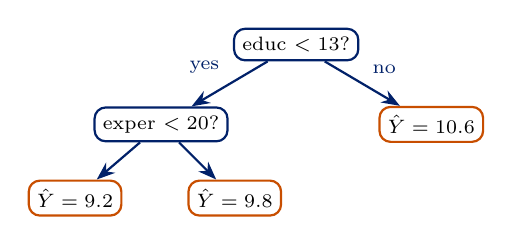
\begin{tikzpicture}[scale=0.78,>=Stealth,thick,font=\scriptsize]
  \node[draw=dukeblue,rounded corners,inner sep=3pt] (r) at (0,2.4) {educ $< 13$?};
  \node[draw=dukeblue,rounded corners,inner sep=3pt] (l) at (-2.2,1.1) {exper $< 20$?};
  \node[draw=accent,rounded corners,inner sep=3pt] (rr) at (2.2,1.1) {$\hat Y = 10.6$};
  \node[draw=accent,rounded corners,inner sep=3pt] (ll) at (-3.6,-0.1) {$\hat Y = 9.2$};
  \node[draw=accent,rounded corners,inner sep=3pt] (lr) at (-1.0,-0.1) {$\hat Y = 9.8$};
  \draw[->,dukeblue] (r)--(l) node[midway,above left]{yes};
  \draw[->,dukeblue] (r)--(rr) node[midway,above right]{no};
  \draw[->,dukeblue] (l)--(ll); \draw[->,dukeblue] (l)--(lr);
\end{tikzpicture}
\end{center}
\vskip-4pt
\begin{itemize}\itemsep2pt
  \item \textbf{Strengths}: automatic interactions and nonlinearity; invariant to
        monotone transformations; handles mixed variable types; readable.
  \item \alert{Weaknesses}: high variance --- a small change in the data can
        change the first split and hence everything below it. A single deep tree
        overfits badly; a shallow one underfits.
  \item Pruning with a complexity penalty helps but does not solve it. The real
        fix is to average many trees.
\end{itemize}
\end{frame}

\begin{frame}{Bagging, Random Forests, Boosting}
\begin{itemize}\itemsep4pt
  \item \textbf{Bagging}: fit trees on bootstrap resamples and average. Averaging
        $B$ nearly independent estimates cuts variance by roughly $1/B$ without
        adding bias. But bootstrap trees are \emph{correlated} --- they all split
        on the same dominant predictor first --- which caps the gain.
  \item \textbf{Random forests}: bag, but at each split consider only a random
        subset of $m$ predictors. Decorrelating the trees is what makes the
        averaging work. $m$ is the main tuning parameter, alongside node size.
        Out-of-bag error is a free cross-validation estimate.
  \item \textbf{Boosting}: fit trees \emph{sequentially}, each on the residuals of
        the current ensemble, adding a shrunken version:
        $\hat f \leftarrow \hat f + \eta\,\hat t$. Attacks \emph{bias} rather than
        variance, and with small $\eta$ and many trees is usually the strongest
        tabular predictor available.
\end{itemize}
\vskip3pt
\alert{Bagging and random forests reduce variance; boosting reduces bias.} That
is the cleanest way to keep them straight.
\end{frame}

\begin{frame}{What ML Buys, and What It Does Not}
\begin{columns}[T]
\begin{column}{0.47\textwidth}
\textbf{Buys}
\begin{itemize}\small\itemsep2pt
  \item Prediction with many predictors, including $p > n$.
  \item Automatic nonlinearity and interactions --- no functional form to guess.
  \item Honest out-of-sample performance estimates.
\end{itemize}
\end{column}
\begin{column}{0.49\textwidth}
\textbf{Does not buy}
\begin{itemize}\small\itemsep2pt
  \item \alert{Causal interpretation.} A variable importance score is not an
        effect.
  \item Valid standard errors for the coefficients it selects.
  \item Extrapolation: trees cannot predict outside the training range at all.
  \item Freedom from the identification problems of Weeks 5--11.
\end{itemize}
\end{column}
\end{columns}
\vskip5pt
\begin{block}{The genuine sociological uses}
\emph{Prediction as the goal} (screening, triage, forecasting);
\emph{measurement} (constructing variables from text or images);
\emph{describing heterogeneity}; and \alert{estimating nuisance functions inside a
causal estimator} --- which is next week.
\end{block}
\end{frame}

\begin{frame}{Looking Ahead}
\begin{itemize}\itemsep4pt
  \item Every method today trades bias for variance, tuned by cross-validation.
  \item That trade is exactly why we cannot drop these estimates into a regression
        and read off a coefficient: they are \emph{deliberately biased} and
        converge slowly.
  \item \textbf{Next week}: what has to change before an estimate this biased can
        be used as an ingredient in a causal estimator --- and what it buys us when
        it can.
\end{itemize}
\vskip4pt
\begin{block}{Reading}
ISL Chapters 5, 6, and 8; Molina and Garip (2019). Optional: ISL Chapter 10
(deep learning); Kleinberg et al.\ (2015) on prediction policy problems.
\end{block}
\end{frame}

\begin{frame}{References}
\footnotesize
\begin{itemize}\itemsep3pt
\item James, Gareth, Daniela Witten, Trevor Hastie, and Robert Tibshirani. 2021.
\textit{An Introduction to Statistical Learning}, 2nd ed. Springer. [Ch.\ 5, 6, 8]
\item Kleinberg, Jon, Jens Ludwig, Sendhil Mullainathan, and Ziad Obermeyer.
2015. ``Prediction Policy Problems.'' \textit{American Economic Review: Papers \&
Proceedings} 105(5): 491--495.
\item Molina, Mario and Filiz Garip. 2019. ``Machine Learning for Sociology.''
\textit{Annual Review of Sociology} 45(1): 27--45.
\item Hastie, Trevor, Robert Tibshirani, and Jerome Friedman. 2009.
\textit{The Elements of Statistical Learning}, 2nd ed. Springer.
\item Athey, Susan and Guido W. Imbens. 2019. ``Machine Learning Methods That
Economists Should Know About.'' \textit{Annual Review of Economics} 11: 685--725.
\end{itemize}
\end{frame}

\end{document}
